% Graphical methodology - Objetivo 1
% SAM → QGIS → Embeddings AEF → Clasificación RF

\documentclass[border=1cm]{standalone}
\usepackage[utf8]{inputenc}
\usepackage{tikz}
%\usetikzlibrary{shapes.geometric, arrows, positioning}
\usetikzlibrary{shapes.geometric, arrows.meta, positioning}


% Estilos (como en template.tex)
\tikzstyle{startstop} = [
  rectangle, rounded corners, minimum width=4cm, minimum height=1.6cm,
  text centered, align=center, draw=black, fill=red!30
]
\tikzstyle{process} = [
  rectangle, minimum width=4cm, minimum height=1.6cm,
  text centered, align=center, draw=black, fill=orange!30
]
\tikzstyle{data} = [
  trapezium, trapezium left angle=70, trapezium right angle=110,
  minimum width=4cm, minimum height=1.6cm,
  text centered, align=center, draw=black, fill=blue!25
]
\tikzstyle{decision} = [
  diamond, aspect=1, text centered, align=center,
  draw=black, fill=yellow!35, minimum width=1cm, minimum height=1cm
]
%\tikzstyle{arrow} = [thick,->,>=stealth]
\tikzset{
  arrow/.style={
    very thick,
    -{Stealth[length=7mm,width=4mm]}
  }
}

\begin{document}

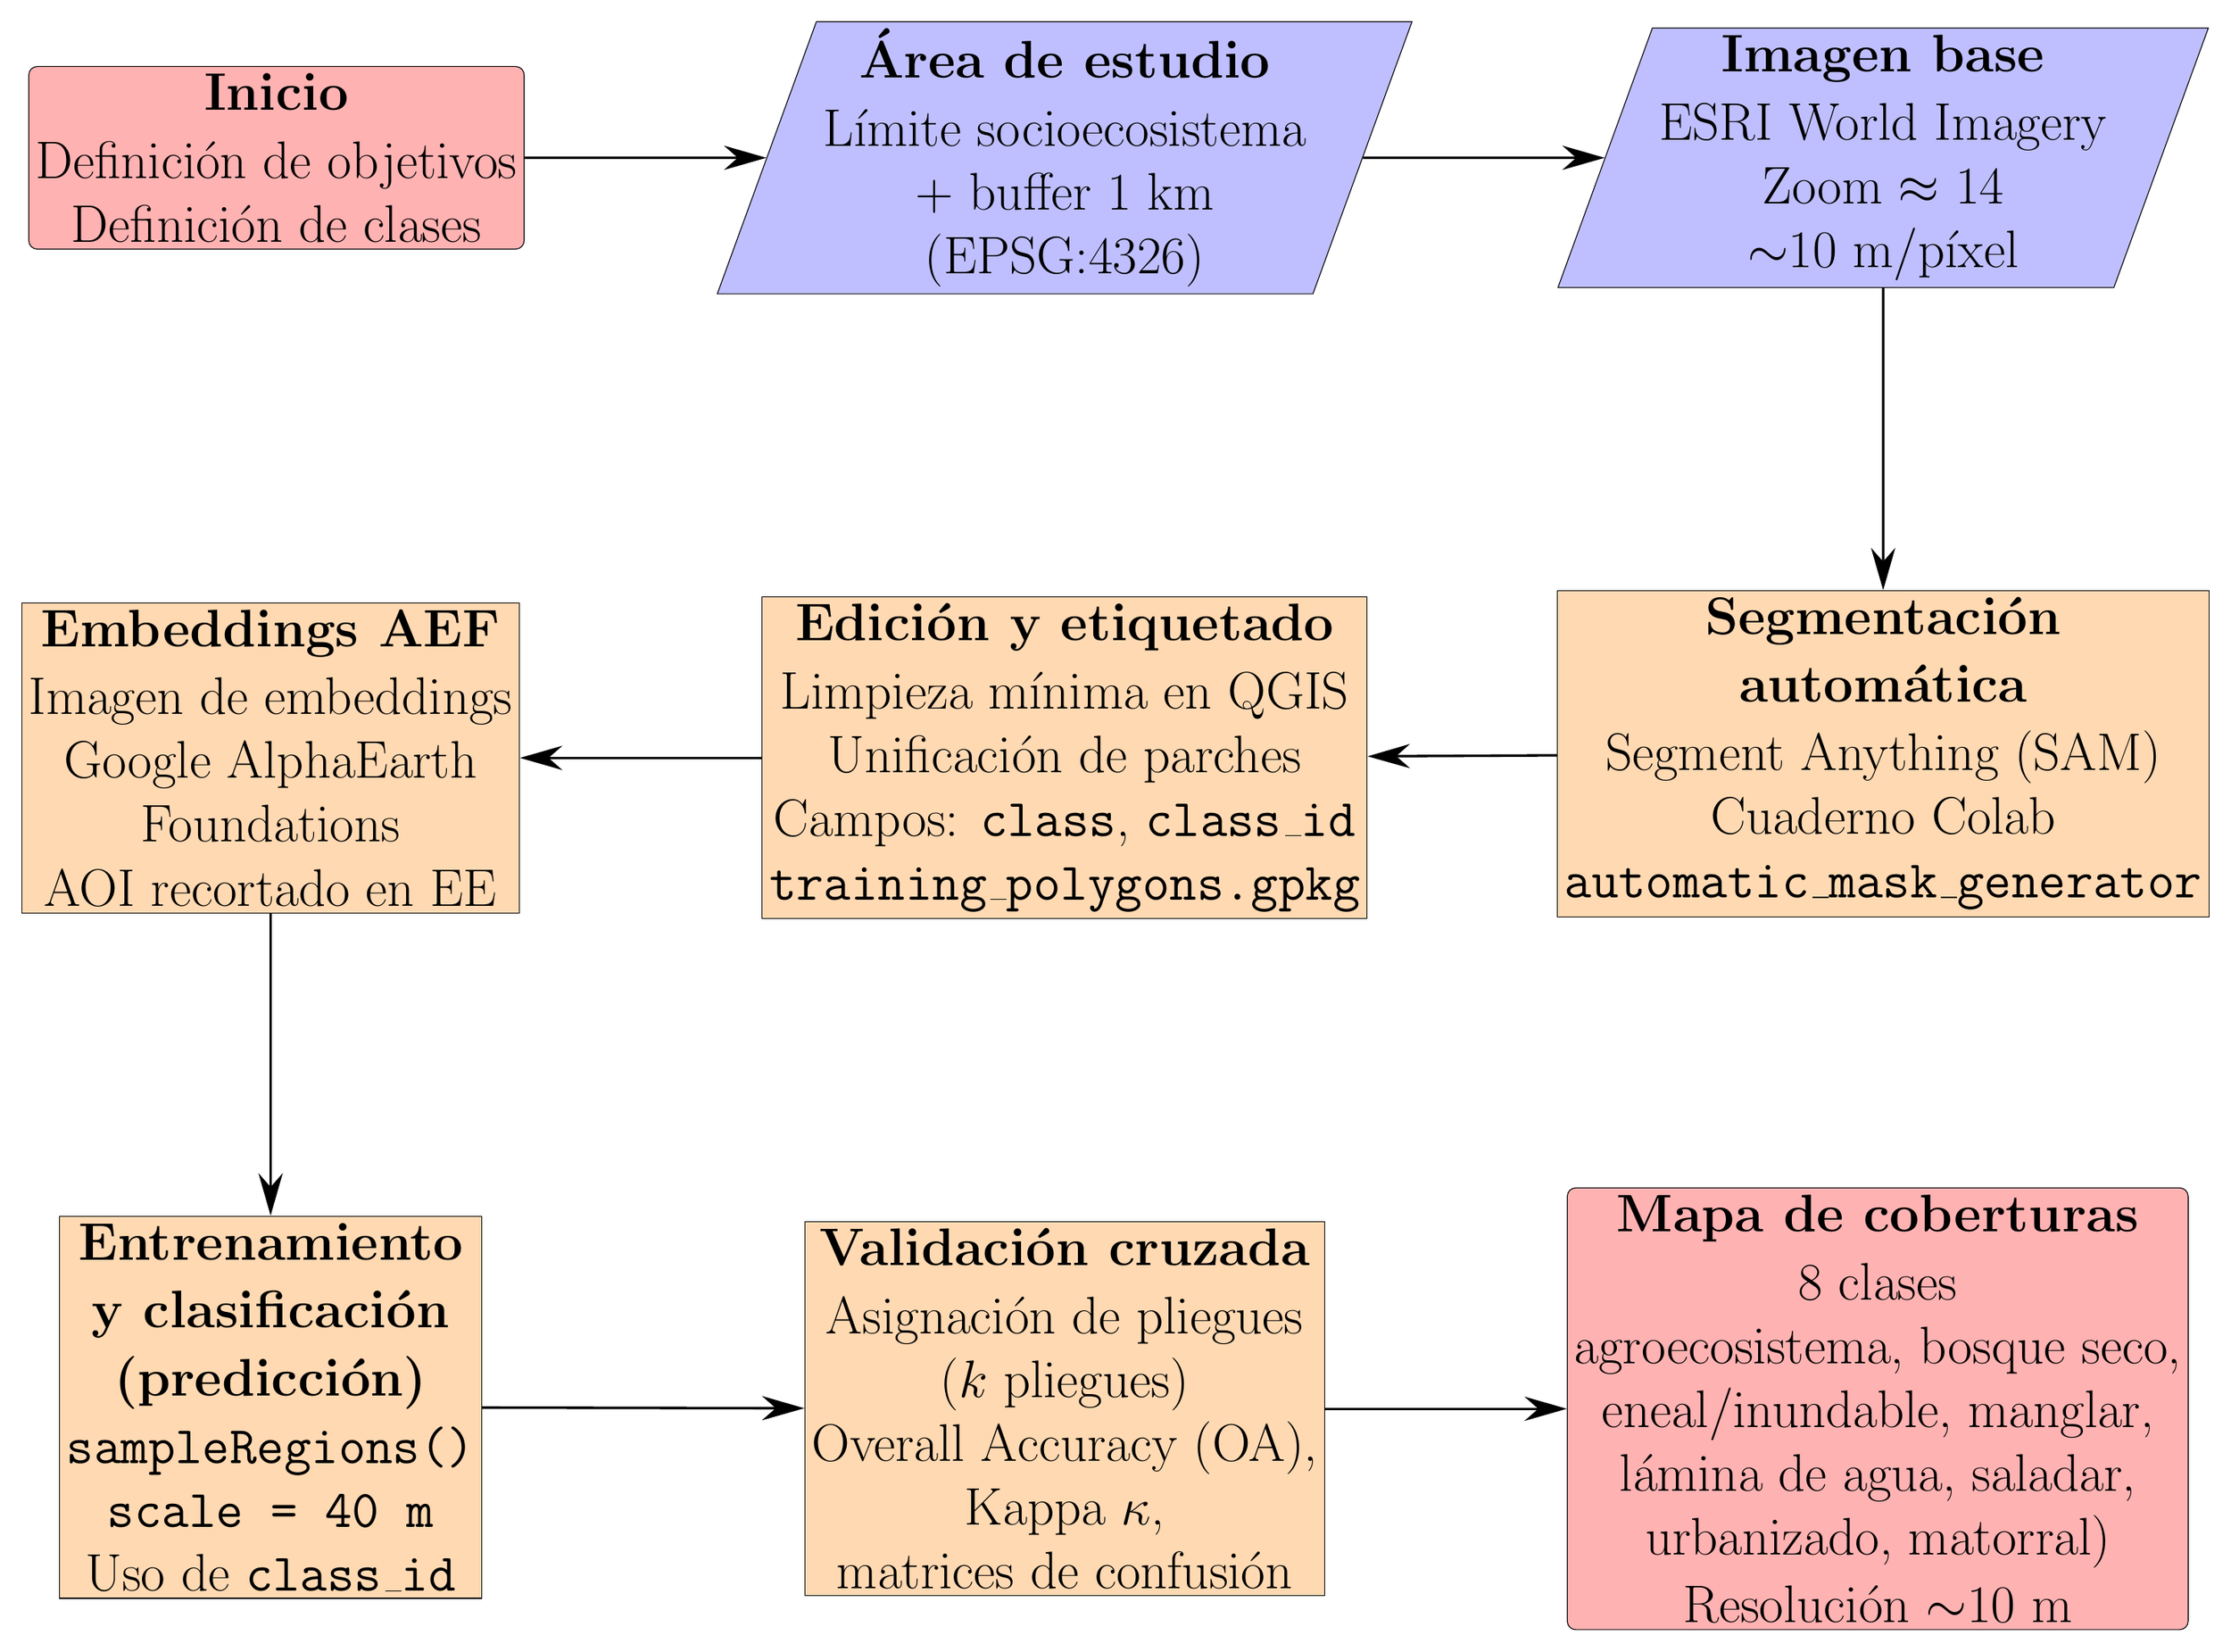
\begin{tikzpicture}[
%  font=\sffamily\footnotesize,
  node distance=5cm and 4cm,
  font=\Huge
%  every node/.style={font=\sffamily\huge}
]

% ------------------------------------------------
% FILA 1 (arriba) – Datos de entrada y máscaras
% ------------------------------------------------

\node[startstop] (n0) {%
  \textbf{Inicio}\\[2pt]
  Definición de objetivos \\
  Definición de clases
};

\node[data, right=of n0] (n1) {%
  \textbf{Área de estudio}\\[2pt]
  Límite socioecosistema\\
  + buffer 1 km\\
  (EPSG:4326)
};

\node[data, right=of n1] (n2) {%
  \textbf{Imagen base}\\[2pt]
  ESRI World Imagery\\
  Zoom $\approx$ 14\\
  $\sim$10 m/píxel
};

% ------------------------------------------------
% FILA 2 (abajo) – Embeddings, clasificación y mapa
% ------------------------------------------------

\node[process, below=of n2] (n3) {%
  \textbf{Segmentación}\\[2pt]
  \textbf{automática}\\[2pt]
  Segment Anything (SAM)\\
  Cuaderno Colab\\
  \texttt{automatic\_mask\_generator}
};

\node[process, below=of n1] (n4) {%
  \textbf{Edición y etiquetado}\\[2pt]
  Limpieza mínima en QGIS\\
  Unificación de parches\\
  Campos: \texttt{class}, \texttt{class\_id}\\
  \texttt{training\_polygons.gpkg}
};

\node[process, left=of n4] (n5) {%
  \textbf{Embeddings AEF}\\[2pt]
  Imagen de embeddings\\
  Google AlphaEarth \\
  Foundations\\
  AOI recortado en EE
};

% ------------------------------------------------
% FILA 3 (abajo)
% ------------------------------------------------

\node[process, below=of n5] (n6) {%
  \textbf{Entrenamiento}\\[2pt]
  \textbf{y clasificación}\\[2pt]
  \textbf{(predicción)}\\[2pt]
  \texttt{sampleRegions()}\\
  \texttt{scale = 40 m}\\
  Uso de \texttt{class\_id}
};

\node[process, below=of n4] (n7) {%
  \textbf{Validación cruzada}\\[2pt]
  Asignación de pliegues\\
  ($k$ pliegues)\\
  Overall Accuracy (OA),\\
  Kappa $\kappa$,\\
  matrices de confusión
};

\node[startstop, right=of n7] (n8) {%
  \textbf{Mapa de coberturas}\\[2pt]
  8 clases \\
  agroecosistema, bosque seco,\\
  eneal/inundable, manglar,\\
  lámina de agua, saladar,\\
  urbanizado, matorral)\\[2pt]
  Resolución $\sim$10 m
};

% ------------------------------------------------
% FLECHAS HORIZONTALES
% ------------------------------------------------

\draw[arrow] (n0) -- (n1);
\draw[arrow] (n1) -- (n2);

\draw[arrow] (n3) -- (n4);
\draw[arrow] (n4) -- (n5);

\draw[arrow] (n6) -- (n7);
\draw[arrow] (n7) -- (n8);

% ------------------------------------------------
% FLECHAS VERTICALES (conexión entre filas)
% ------------------------------------------------

\draw[arrow] (n2) -- (n3);
\draw[arrow] (n5) -- (n6);


\end{tikzpicture}

\end{document}
